\section{Frame invariance and an information leak in a fixed-origin simulation}
\label{app:leak}
Simulations frequently place the lens at the coordinate origin. If absolute image coordinates are then given to a trained estimator, it can measure the image radii from the exact lens center and so bypass the error of the measured center: the inputs contain information that real data do not provide. We quantified this effect on an earlier, smaller benchmark of 2500 selected SIS events (ET-D, $0.05<z_s<1.5$) in which the true center was fixed at the origin and the inputs contained absolute image and center coordinates. With otherwise identical HistGB settings and ten random divisions into training, calibration and test events (1750/375/375), replacing the absolute coordinates by translation-invariant inputs raised the MAE of the geometry-only estimate from $0.193\pm0.038$ to $0.270\pm0.040$, and that with all inputs from $0.207\pm0.041$ to $0.239\pm0.036$. A Bayesian SIS posterior from the image coordinates, marginalized over the unknown center, attains MAE $0.243\pm0.032$ on the same events: it beats the corrected estimator, as it should for a correct lens model, whereas the estimator with absolute coordinates appeared to beat it. In the same earlier study, images in the non-SIS benchmark had been ordered by their true magnification, which reveals the target whenever more than two images exist. All results in this paper use a random true center and frame rotation, inputs that are invariant under translations and rotations, and images ordered by measured SNR.

\section{Additional results}
\label{app:extra}
Fig.~\ref{fig:learning} shows the median relative error as a function of the number of training events for SIS and SIE+shear lenses (ET). The errors stop decreasing above $\sim10^4$ events. The results are therefore not limited by the size of the ET training sets (36\,000 events per family), while the O5 samples (900--1800 training events per family) lose about 1--2 percentage points relative to the asymptotic accuracy.

\begin{figure}
\centering
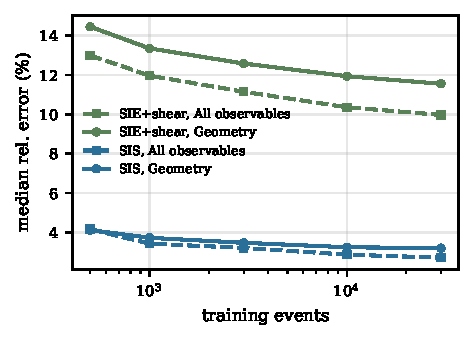
\includegraphics[width=\columnwidth]{fig_learning.pdf}
\caption{Median relative error of $\mu_A$ versus the number of training events for ET.}
\label{fig:learning}
\end{figure}


\section{Likelihoods of the Bayesian lens reconstruction}
\label{app:gwemlike}
This appendix specifies the analyses of Sec.~\ref{sec:gwem}. The lens parameters are $\boldsymbol\eta=(\sigma_v,x_c,y_c,q,\phi_q,\gamma_{\rm ext},\phi_{\rm ext},\gamma')$, with the subset appropriate to each lens model. Their priors are the simulated population distributions: the $\sigma_v^4$-weighted velocity-dispersion function on $100<\sigma_v<400$\,km\,s$^{-1}$, a Gaussian of width 0.02\,arcsec for the lens center relative to the observed light center, $q\sim\mathcal N(0.75,0.15)$ truncated to $[0.35,0.99]$, $\ln\gamma_{\rm ext}\sim\mathcal N(\ln0.05,0.6)$ truncated to $[\ln10^{-3},\ln0.25]$, $\gamma'\sim\mathcal N(2.08,0.15)$ truncated to $[1.6,2.6]$, and uniform position angles. The Einstein radius follows from $\sigma_v$ through the SIS relation at the observed redshifts.

\emph{EM likelihood.} Each observed image position $\boldsymbol\theta_i$, with uncertainty $\sigma_i$, maps to the source plane as $\boldsymbol\beta_i=\boldsymbol\theta_i-\boldsymbol\alpha(\boldsymbol\theta_i;\boldsymbol\eta)$. To first order, a source position $\boldsymbol\beta$ predicts an image displaced from $\boldsymbol\theta_i$ by $A_i^{-1}(\boldsymbol\beta_i-\boldsymbol\beta)$, where $A_i$ is the lensing Jacobian at $\boldsymbol\theta_i$, so that
\begin{equation}
\begin{split}
-2\ln\mathcal L_{\rm pos}(\boldsymbol\eta,\boldsymbol\beta)={}&\sum_i(\boldsymbol\beta_i-\boldsymbol\beta)^{\rm T}W_i(\boldsymbol\beta_i-\boldsymbol\beta)\\
&+\sum_i 2\ln(2\pi\sigma_i^2),
\end{split}
\end{equation}
with $W_i=A_i^{-\rm T}A_i^{-1}/\sigma_i^2$.
Integrating over $\boldsymbol\beta$ with a flat prior gives
\begin{equation}
\begin{split}
\ln\mathcal L_{\rm pos}(\boldsymbol\eta)={}&-\tfrac12\chi^2_{\rm min}-\tfrac12\ln\det W\\
&+\ln2\pi-\sum_i\ln(2\pi\sigma_i^2),
\end{split}
\end{equation}
with $W=\sum_iW_i$,
where $\chi^2_{\rm min}$ is evaluated at $\hat{\boldsymbol\beta}=W^{-1}\sum_iW_i\boldsymbol\beta_i$; the parameter-dependent normalization $-\frac12\ln\det W$ is retained. The model images are obtained by one Newton step from the observed positions, and the magnifications, Morse indices and Fermat potentials of the two GW images are evaluated there. In the exact variant, used as a check in Sec.~\ref{sec:gwem} and for coarse astrometry in Sec.~\ref{sec:discussion}, the source position is sampled as $\boldsymbol\beta=\hat{\boldsymbol\beta}+L\boldsymbol u$, with $LL^{\rm T}=W^{-1}$ and $\boldsymbol u$ uniform in $[-8,8]^2$; each model image is found by iterating the lens equation to convergence from the observed position, and $\ln\mathcal L_{\rm pos}=-\frac12\sum_i|\boldsymbol\theta_i^{\rm model}-\boldsymbol\theta_i|^2/\sigma_i^2-\sum_i\ln(2\pi\sigma_i^2)+\ln\det L$, where the last term makes the prior flat in $\boldsymbol\beta$. The EM likelihood multiplies $\mathcal L_{\rm pos}$ by Gaussians for the light axis ratio (width 0.05), the light position angle (width $10\degr$) and the measured velocity dispersion (width $0.1\sigma_v$).

\emph{Source-position prior.} A flat prior on $\boldsymbol\beta$ with the same normalization for every lens model does not reproduce the simulated population. The simulation draws the source uniformly in area within a disk of radius $R\,\theta_E$ ($R=1$ for the SIS, 1.6 for the SIE and 1.8 for the models with shear) and redraws it, up to 60 times, until the lens produces at least two images; after 60 failures the lens itself is redrawn. For a given lens the source density is therefore $1/A_{\rm mult}$ over the multiple-image region, the set of source positions that produce at least two images, whose area is $A_{\rm mult}=a\,\pi(R\theta_E)^2$, where $a(\boldsymbol\eta)$ is the fraction of the disk inside that region. The lens is retained with probability $1-(1-a)^{60}$. We therefore multiply the EM likelihood by $[1-(1-a)^{60}]/A_{\rm mult}$. The fraction $a$ is computed with the image solver and acceptance test of the simulation on a fixed set of 1200 source positions, tabulated on a grid in $\gamma'$, $q$, $\gamma_{\rm ext}$ and the angle between the shear and the mass major axis, and interpolated between grid points ($a=1$ for the SIS). Without this factor the posterior weights each lens model by $A_{\rm mult}$, which grows steeply with the slope. For $q=0.75$ and $\gamma_{\rm ext}=0.05$, $a=0.09$, 0.30 and 0.84 at $\gamma'=1.8$, 2.0 and 2.2, because a steeper profile forms a faint central image even for sources well outside the Einstein radius. The omission therefore favors steep slopes and underestimates $\mu_A$. We tested this on 143 EPL+shear systems drawn from the population without any detection requirement and analyzed with the EM data alone. Without the factor the posterior mean slope exceeds the true slope by $0.050\pm0.011$ on average, the median of $\ln\mu_A$ is low by $0.106\pm0.023$, and the 90\% credible intervals contain the true slope and $\mu_A$ in 87\% of the systems. With the factor the offsets are $-0.014\pm0.011$ and $-0.022\pm0.023$, the intervals contain the true values in 93\% and 90\%, and the fraction of posterior samples below the true value is consistent with a uniform distribution, as expected for calibrated posteriors (Kolmogorov--Smirnov $p=0.62$ for the slope and 0.98 for $\ln\mu_A$, compared with $p\le0.001$ without the factor). All results in Sec.~\ref{sec:gwem} include the factor.

\emph{GW quantities predicted by the lens.} For the known image assignment, the lens model predicts $\mu_A=|\mu_a|$, the ratio $R=|\mu_b/\mu_a|$, the Morse indices $n_A$, $n_B$, and the Fermat-potential difference $\Delta\phi$. Without a cosmology, the GW data constrain only $R$, $n_A$, $n_B$ and the arrival order: $\Delta\phi$ must have the sign of the measured delay, and the dimensional delay and the apparent distance remain free nuisance parameters.

\emph{Two-stage analysis.} The joint-PE posterior $p(\boldsymbol\xi|d)$, with GW parameters $\boldsymbol\xi$, is converted into an effective likelihood for the quantities the lens predicts, $\mathcal L_{\rm eff}(\ln R,\ln D_{{\rm app},A},n_A,n_B)\propto p(\ln R,\ln D_{{\rm app},A},n_A,n_B|d)/\pi_{\rm PE}$. The PE priors are uniform in $\ln R$ and in the Morse indices and $\propto D_{{\rm app},A}^2$ in distance; the other GW parameters (masses, spins, sky position, orientation, phase, arrival time and delay) are marginalized under their PE priors, which do not depend on the lens. We approximate $\mathcal L_{\rm eff}$ by a two-dimensional Gaussian in $(\ln R,\ln D_{{\rm app},A})$, fitted to the posterior samples with weights $D_{{\rm app},A}^{-3}$ (which remove the distance prior and convert to $\ln D$), multiplied by the marginal posterior probabilities of the nine Morse combinations, $P(n_A,n_B)=(k+0.5)/(N+4.5)$ for $k$ of $N$ samples. This product neglects any dependence of the $\ln R$ distribution on the Morse combination. In the PE posteriors the conditional means of $\ln R$ for different combinations differ from the overall mean by a median 0.03 (ET, host sky position) and 0.05 (O5) posterior standard deviations, with 90th percentiles of 0.08 and 0.19. Because no cosmology is assumed, only the $\ln R$ marginal is used.
